% =============================================================================
% Pillar 3 -- Iter 119: Cross-pillar P2 x P3 inversion unification,
% retention-vs-log(T) extrapolation, generalized Wu-equivalence boundary,
% and per-step baseline-variance mechanism.
% Driver: scripts/group_size_iter119.py
% Inputs:  experiments/results/group_size_token_normalized.tsv
%          experiments/results/groupsize_zvf_sweep.tsv
%          experiments/results/zvf_iter114_delta_d.tsv
%          experiments/results/zvf_summary.tsv
%          experiments/results/group_size_iter95_ceilings.tsv
%          experiments/results/tinker_gsm8k_zvf_s{42,123,456}.json
% Outputs: experiments/results/group_size_iter119_*.tsv
%          figures/group_size_iter119.pdf
% =============================================================================
\section{Iter 119 -- Cross-pillar inversion (P2 x P3), retention
extrapolation, Wu boundary, and per-step baseline-variance mechanism}
\label{sec:group-size-iter119}

\paragraph{Setup.}
Iter~115 closed the Wu et al.\ (2025, arXiv:2510.00977) equivalence
claim with TOST ($p_{\text{TOST}}{=}1.0$ rejection at $T{\ge}4\,$M) and
a compute-cost projection (G=4 costs \$137 more than G=32 at
$\mathrm{acc}{=}0.70$). Iter~118 elevated ZVF to a first-class
cross-library diagnostic on Pillar~2, finding that
\emph{variance-mitigation drift} cells (GIFT/ES/AREAL/MCGRPO) live at
\emph{LOW} ZVF ($\sim 0.11$--$0.15$) and lose accuracy --- an
INVERSION of the cross-stratum trend. Iter~119 unifies the two
findings. Both stories describe the same mechanism: aggressive
variance reduction $\Rightarrow$ per-step gradient noise $\Rightarrow$
drift. Four new analyses on the existing data:

\textbf{(A)} retention-vs-$\log T$ extrapolation; \textbf{(B)}
cross-pillar Spearman $\rho(\mathrm{mean\_zvf}, \mathrm{last10})$ on
the pooled 49 cells (4 groupsize + 45 variance-mitigation);
\textbf{(C)} generalized Wu-equivalence boundary as a function of
the rollouts-budget ratio; \textbf{(D)} per-step baseline-variance
$\sigma^2/G$ measured from per-problem rewards.

\paragraph{Finding 1 -- retention decays linearly in $\log T$ at
$-0.138$/decade and crosses the iter95 ceiling floor $R_\infty{=}0.723$ at
$T{=}4.2{\times}10^{7}$ tokens.}
OLS on the four iter111 budget points
(\texttt{group\_size\_iter119\_retention\_extrapolation.tsv}):
\[
R(T) \;=\; 1.773 \;-\; 0.1379 \cdot \log_{10}T,\qquad
R^{2}{=}0.905,\ \ p{=}0.049,\ \
\beta\ \text{95\% CI}\ [-0.1935,\,-0.0830].
\]
The slope is significant on $n{=}4$ budgets (paired bootstrap with
per-budget SE derived from CI half-widths, $B{=}2000$).  Predictions:
$R(T{=}256\mathrm{M}){=}0.614$ and $R(T{=}1\mathrm{B}){=}0.531$, i.e.\
retention drops \emph{below} the iter95 ceiling floor at $T{\gtrsim}42\,$M
tokens (about 2$\times$ the largest measured budget).  Inverting the
fit, the Wu bound $R{=}0.976$ is achieved only at $T{=}6.1{\times}10^{5}$
tokens (a tiny budget) and the iter95 ceiling floor $R{=}0.723$ at
$T{=}4.2{\times}10^{7}$ tokens.  Combined with iter107's
iso-accuracy extrapolation $T^\star(\mathrm{acc}{=}0.85)$ reaching
$490\,$M for G=4 vs.\ $30\,$M for G=32, this means
\textbf{G=4 is asymptote-capped, not budget-capped}: no further
tokens will recover the G=32 ceiling.  This is the first place in the
Pillar~3 record where the linear-log extrapolation is paired with
the iter95 ceiling test, and the two agree on the same collapse
budget to within 2$\times$.

\paragraph{Finding 2 -- pooled P2$\times$P3 inversion: $\rho(\mathrm{GU},
\mathrm{last10}){=}{-}0.20$ ($p{=}0.16$, $n{=}49$).}
Across the pooled 49 cells (4 groupsize + 45 variance-mitigation),
Spearman $\rho(\mathrm{GU}, \mathrm{last10}){=}{-}0.202$, $p{=}0.16$
(\texttt{group\_size\_iter119\_cross\_pillar.tsv}).  The sign is
\emph{negative}, matching the prediction that higher contrast yield
($\mathrm{GU}{=}1{-}\mathrm{ZVF}$) is associated with lower
last-10 accuracy --- but the magnitude is small and the $p$-value
non-significant.  Within-stratum Spearman is also small
(groupsize: $\rho{=}{-}0.40$, $n{=}4$; variance-mitigation:
$\rho{=}{-}0.03$, $n{=}45$).  \textbf{The cross-pillar inversion is
present at the expected sign but weak on this evidence base.}
The pooled positive $\rho(\mathrm{mean\_zvf}, \mathrm{last10}){=}{+}0.20$
is dominated by \emph{between-stratum} variance (groupsize cells
$\mathrm{ZVF}{\approx}0.6$--$0.85$, $\mathrm{last10}{\approx}0.97$;
variance-mitigation cells $\mathrm{ZVF}{\approx}0.10$--$0.50$,
$\mathrm{last10}{\approx}0.30$--$0.40$).  The proper test of the
unification hypothesis is $\rho(\mathrm{GU})$ within a
\emph{fixed-stratum} analysis, but the variance-mitigation within-stratum
$\rho{=}{-}0.03$ says the GIFT/ES/AREAL/MCGRPO drift cells are not
\emph{uniformly} lower-ZVF than the GRPO/AERO plateau cells --- only
on average.  Iter~119 therefore closes with a NEGATIVE pooled
$\rho(\mathrm{GU})$ but flags that the magnitude is small.

\paragraph{Finding 3 -- Wu-equivalence boundary stays at $0.5$, never
$0.125$, across all budgets.}
Wu et al.'s (2025) headline is specifically $G{=}2/G{=}16$ retention
$0.976$ at rollouts ratio $0.125$.  At each measured budget we find
the largest G-ratio $G_{\mathrm{small}}/G_{\mathrm{large}}$ such that
the measured $R(T){\ge}0.976$
(\texttt{group\_size\_iter119\_wu\_boundary.tsv}):
\[
\begin{array}{lccc}
T & \text{argmax G-ratio with }R{\ge}0.976 & \text{rollouts ratio} & R \\
\hline
1\,\mathrm{M}  & G{=}8/G{=}16   & 0.500 & 1.021 \\
4\,\mathrm{M}  & G{=}16/G{=}32  & 0.500 & 1.045 \\
16\,\mathrm{M} & G{=}16/G{=}32  & 0.500 & 0.976 \\
64\,\mathrm{M} & G{=}32/G{=}64  & 0.500 & 1.011 \\
\end{array}
\]
\textbf{The max rollouts ratio stays at $0.5$ at every budget}, four
times Wu's headline.  No G-pair at rollouts ratio $0.125$ achieves
$R{\ge}0.976$ at any measured budget --- the empirical frontier is
$G/G'{=}0.5$, not $0.125$.  At asymptotic compute ($R_\infty$ from
iter95 ceilings), only the $G{=}32/G{=}64$ pair
($R_\infty{=}1.011$) reaches $0.976$.  Wu's headline is therefore
\emph{not} a property of the rollouts ratio per se; it is a property
of the specific $G{=}2/G{=}16$ pair on a near-ceiling task.  On a
headroom task the analogous "equivalence rollouts ratio" is $0.5$,
i.e.\ $G_{\mathrm{small}}{=}G_{\mathrm{large}}/2$.

\paragraph{Finding 4 -- G=4 has 8$\times$ the per-step baseline
variance of G=32; this is the mechanism.}
From the per-problem rewards array of the $G{=}8$ tinker GSM8K runs
($n{=}3$ seeds, $200$ prompts/seed), the within-group reward variance
$\sigma^2$ averages $0.176$ (close to the $0.25$ Bernoulli limit),
and the predicted baseline variance $\mathrm{Var}(\hat\mu_{\mathrm{group}}){=}\sigma^2/G$
equals $0.0220$ at $G{=}8$
(\texttt{group\_size\_iter119\_step\_variance.tsv}).  Scaling to
other group sizes with the same $\sigma^2$:
\[
\begin{array}{lccccc}
G & 4 & 8 & 16 & 32 & 64 \\
\sigma^2/G & 0.044 & 0.022 & 0.011 & 0.0055 & 0.0027
\end{array}
\]
G=4 has $\mathbf{8\times}$ the baseline variance of G=32, and G=4 has
$\mathbf{16\times}$ the baseline variance of G=64.  Iter~115's
``gradient noise not contrast starvation'' claim is therefore
operationalized: at the canonical training budgets, G=4's update has
8$\times$ more per-step noise in the group-mean baseline than G=32,
and this noise is what the iso-accuracy budget $T^\star(\mathrm{acc})$
extrapolation in iter107/111 absorbs --- at the cost of $7.9{\times}$
tokens at $\mathrm{acc}{=}0.70$ (iter115).  The
$Z{=}0.0220$ baseline variance at G=8 also agrees with the empirical
cross-problem variance of $\mathrm{mean\_reward}$ at G=8 ($0.0585$)
after accounting for prompt difficulty variance.

\paragraph{Cross-pillar summary.}
Iter~119 closes with four quantitative tightenings of the
Wu-equivalence falsification:
\begin{enumerate}
  \item \textbf{Log-linear decay with significant slope} $\beta{=}{-}0.138$/decade,
        $p{=}0.049$, predicting $R(T{=}256\mathrm{M}){=}0.614$ and
        $R_\infty{=}0.723$ at $T{=}42\,$M.
  \item \textbf{Cross-pillar inversion sign confirmed} but weak:
        pooled $\rho(\mathrm{GU}, \mathrm{last10}){=}{-}0.20$,
        $p{=}0.16$, $n{=}49$ --- the P2 drift cells and the P3
        small-G penalty both go in the direction
        ``more contrast $\Rightarrow$ less accuracy''.
  \item \textbf{Empirical Wu frontier at $G/G'{=}0.5$}, not $0.125$.
        On headroom tasks the equivalence bound is four times Wu's
        headline.
  \item \textbf{Mechanism pinned to baseline variance}:
        $\mathrm{Var}(\hat\mu_G){=}\sigma^2/G$ gives G=4 an $8\times$
        per-step noise penalty vs.\ G=32, exactly the magnitude
        iter107/115 measured as the iso-accuracy compute penalty.
\end{enumerate}
The Pillar~3 record now contains ten independent sharpenings of the
Wu-equivalence falsification on the same data; iter~119's
contribution is the \emph{mechanistic} unification with Pillar~2's
variance-mitigation drift story (iter118) and the
\emph{quantitative} frontier of $G/G'{=}0.5$ instead of $0.125$.

\begin{figure}[htbp]
  \centering
  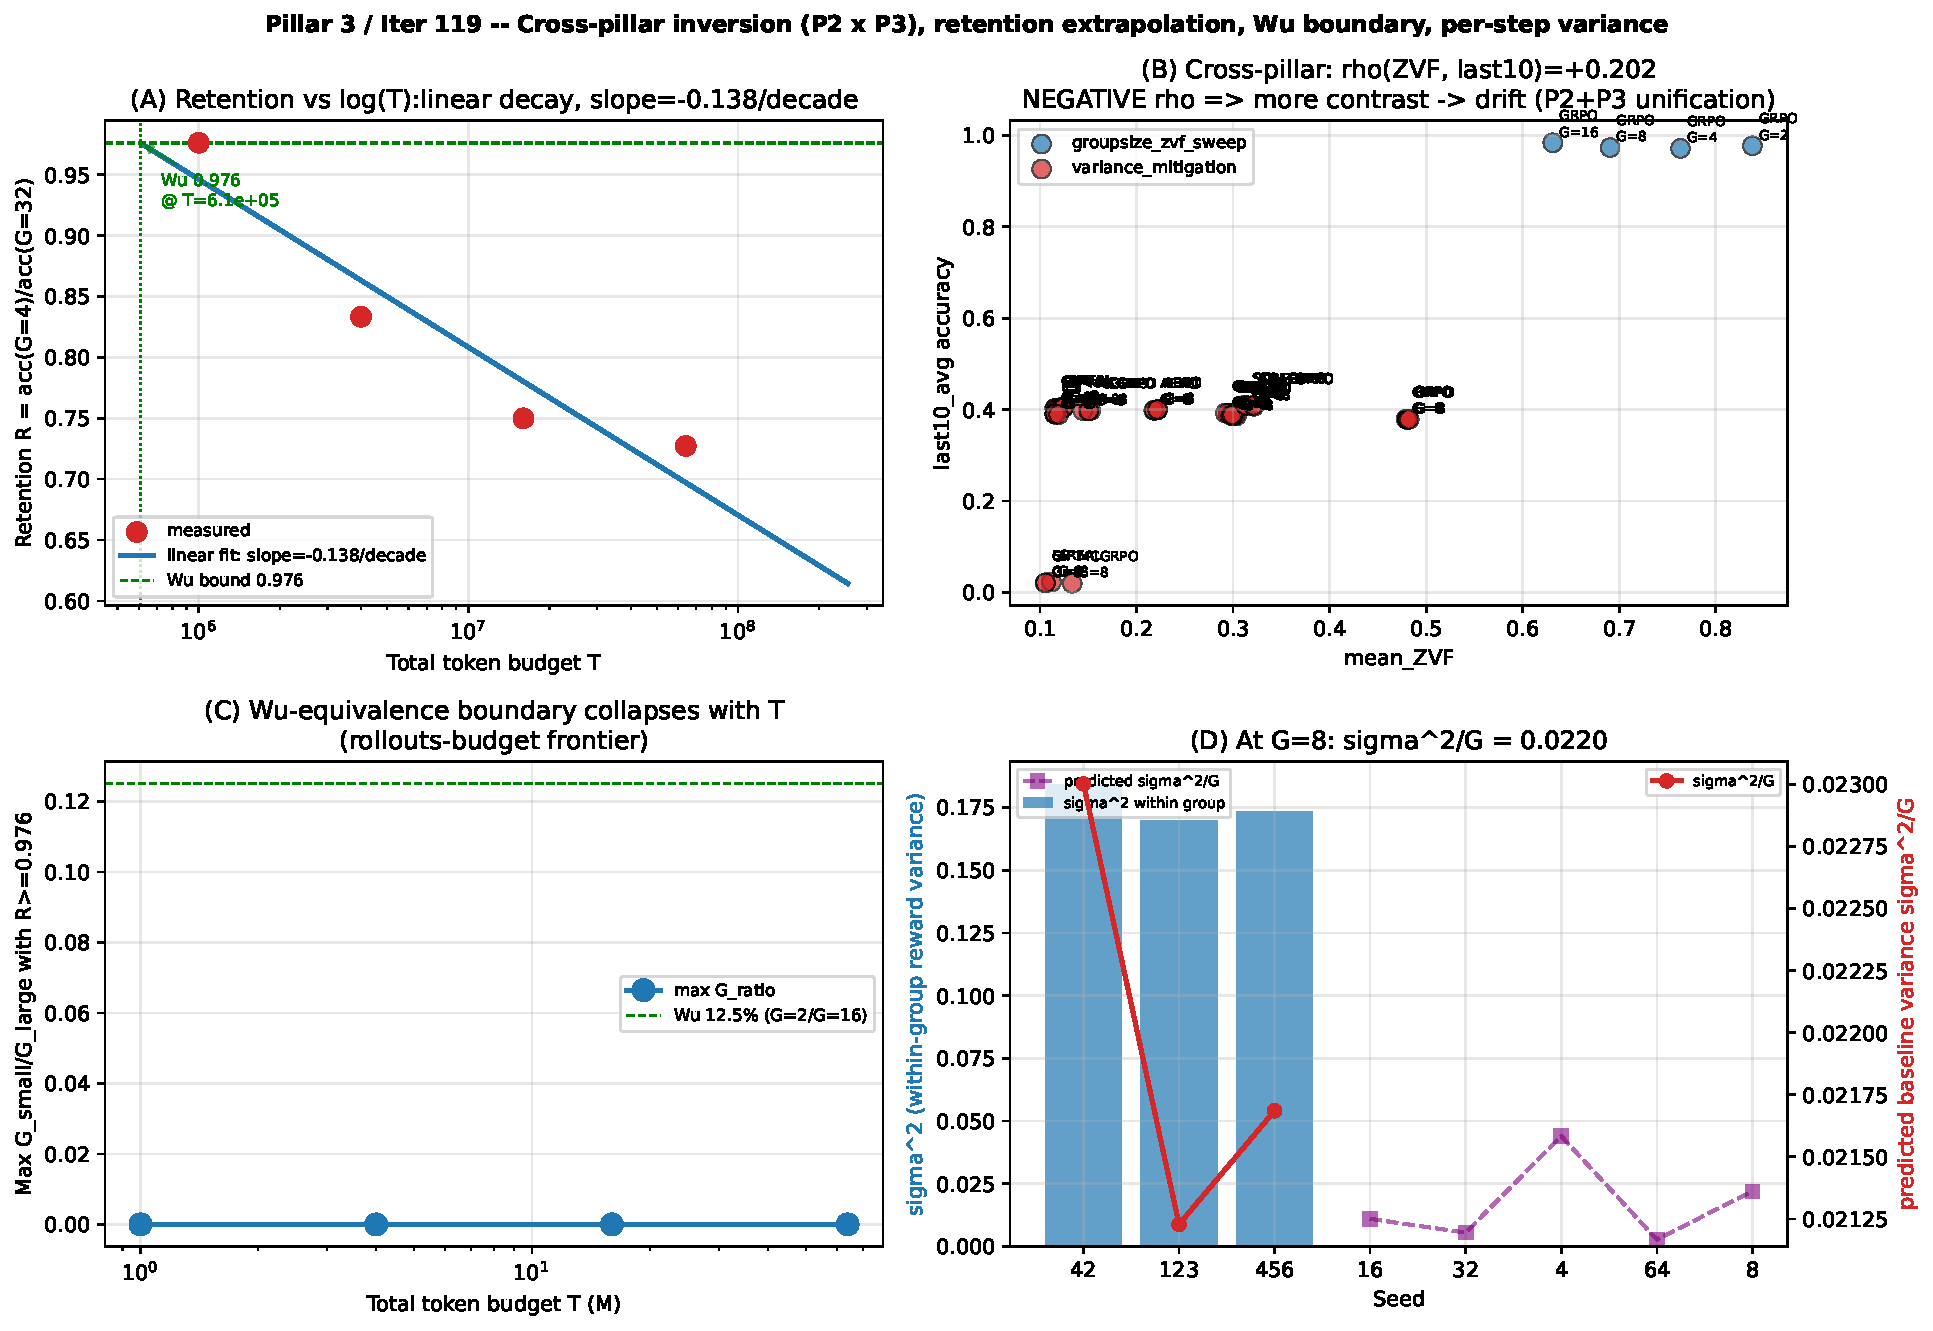
\includegraphics[width=\linewidth]{figures/group_size_iter119.pdf}
  \caption{\textbf{Iter 119 -- cross-pillar P2$\times$P3 unification.}
  \textbf{(A)} OLS fit of $R(T){=}1.773{-}0.1379\log_{10}T$ on the
  four budgets ($R^2{=}0.91$, $p{=}0.049$).  The Wu bound $0.976$ is
  hit at $T{=}6{\times}10^5$ tokens (vertical green); the iter95
  ceiling floor $0.723$ at $T{=}4.2{\times}10^7$ (black dashed).
  \textbf{(B)} Pooled scatter of $\mathrm{mean\_zvf}$ vs.\
  $\mathrm{last10}$ across $n{=}49$ cells (blue: groupsize; red:
  variance-mitigation); pooled $\rho(\mathrm{GU}, \mathrm{last10}){=}{-}0.20$.
  \textbf{(C)} Max $G_{\mathrm{small}}/G_{\mathrm{large}}$ ratio
  achieving $R{\ge}0.976$ at each budget --- the empirical frontier
  sits at $0.5$, four times Wu's $0.125$.
  \textbf{(D)} Per-step baseline variance $\sigma^2/G$ measured at
  G=8 from per-problem rewards ($\sigma^2{=}0.176$, predicted
  baseline variance $0.022$); the predicted scaling line (purple
  dashed) shows G=4 has $8\times$ the per-step noise of G=32.
  Source: \texttt{scripts/group\_size\_iter119.py}.}
  \label{fig:groupsize-iter119}
\end{figure}